\section{Bond Graph representation of oil-market dynamics}
\label{sec: EconEng}

\subsection{crude oil price drivers}
The oil-economic literature identifies multiple factors that affect the price of crude oil.
The US Energy Information Administration (EIA) captures the four most important factors in a simple model \cite{eia}, shown in Figure \ref{fig:EIAmodel}.
The four factors consist of supply, demand, inventory balance, and the financial markets.
An extensive analysis of the EIA model supported by a literature review is provided in \cite{Lang2020}.
In this section, we discuss how the four factors can be modeled with dynamical systems theory resulting in a dynamical systems model for oil prices.




\subsection{Oil Price as momentum, inventory as displacement}
We consider the oil price as a dynamical state.
The oil price changes over time due to the effect of supply, demand, inventories, and financial markets.
We model this as a momentum
\begin{equation}
\label{eq: pdot}
    {p}(t) = \int e(t) dt,
\end{equation}
where $p(t)$ is  the oil price in $\$/\#$ and $e(t)$ is an ''economic effort'' applied by on or more factors in $\$/\#\cdot$ yr.

We model oil inventory as a displacement
\begin{equation}
    \label{eq: qdot}
 q(t) = \int Q (t) dt,
\end{equation}
where $Q(t)$ is the net flow rate of oil in $\#/$yr. 


\subsection{Competitive and OPEC Oil supply}
Oil supply is identified as a driver of the long-term equilibrium price.
Oil supply is typically divided in Organization of the Petroleum Exporting Countries (OPEC) and non-OPEC production.
This division is made because the OPEC members produce with respect to a central coordination and are mostly in hands of national oil companies, whereas non-OPEC producers are mostly in hands of investor-owned companies that make independent decisions.

To make the same distinction between OPEC and non-OPEC members, we will model non-OPEC members as inductive elements and OPEC members as controlled current sources.

\subsubsection{non-OPEC producers}
Non-OPEC oil producers make independent decisions.
In addition, they are assumed to make decisions so as to make return on investments at the actual market price.
We consider non-OPEC producers as inertia elements that produce a flow rate of oil as a function of the current market price.
The relation between production and price is
\begin{equation}
    f_{nOPEC}(p) = \varepsilon_{s} p(t),
\end{equation}
where $\varepsilon_s$ is the elasticity of supply.

The elasticity of supply relates the market price of oil to oil production.
Assuming a competitive market where producers supply at a price close to their marginal costs, the elasticity represents the slope of the marginal cost curve.
In this paper we take a very simplistic view of the oil supply, ignoring non-linear and non-continuous increases of marginal costs that arise from switching to more expensive extraction methods.

\begin{comment}

\begin{equation}
y_i(t) = \begin{cases}
E_i(\lambda(t)-p_{f,i}) & \text{if}\ \lambda\geq p_{f,i}\ \text{and}\ y_i(t) \in Y_i\\
0 & \text{if} \lambda\leq p_{f,i}
\end{cases}
\end{equation}
\end{comment}

\begin{figure}
    \centering
    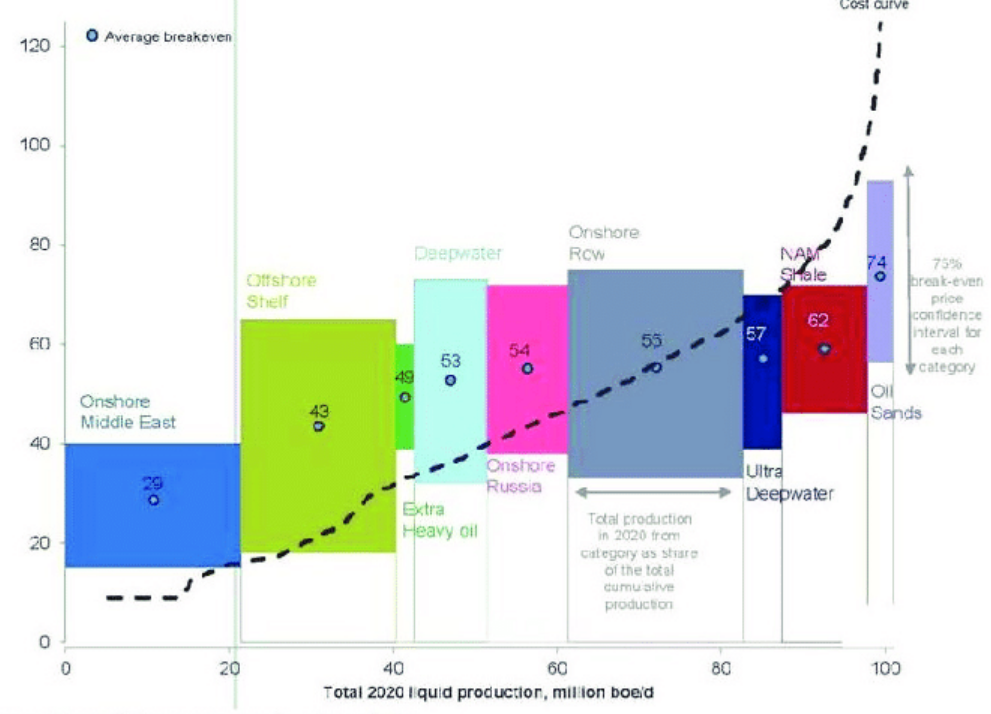
\includegraphics[width=.4\textwidth]{Figures/cost curve.PNG}
    \caption{Marginal cost curve of crude oil as piecewise-affine function}
    \label{fig:marginalcost}
\end{figure}

\subsubsection{OPEC}
OPEC members do not produce according to a free market principle, i.e. basing production levels on the market price.
Instead, the organization sets predetermined production targets for its member countries.
The cost-minimization model used for non-OPEC members thus does not apply to OPEC members.

In this paper, we assume that we cannot derive a model of OPEC's policy.
Hence we consider the supply from OPEC members as a flow source that acts as a disturbance on the oil market.
\begin{equation}
    f_{opec}(t) = d_{opec}(t)
\end{equation}




\subsection{Oil demand}
On the demand side, the EIA model makes a distinction between member states of the Organization of Economic Cooperation and Development (OECD) and non-OECD countries.
Most developed countries, e.g. the US and countries in the European Union, are members of the OECD.
The oil consumption in OECD countries is less dependent on economic growth than for developing countries.
This is because the GDP of developed countries is more stable, tax policies slow down oil consumption, and developed countries have larger service industries relative to manufacturing industries.
As a result, the oil consumption in OECD countries is mostly dependent on the oil price.
\begin{equation}
    f_{OECD} = f_0 - \varepsilon_D p(t)
\end{equation}


Many non-OECD members are developing countries, among which China, India, and Saudi Arabia are the biggest consumers.
In non-OECD counries, oil consumption is stronger related to economic growth rather than to oil prices.
This is a result of on the one hand changing conditions in developing economies, such as increases in population and purchasing power, and on the other hand the higher share of manufacturing industry and use of oil as energy source and feedstock.   
Therefore, non-OECD consumption cannot be modeled like OECD consumption.
Instead, we propose to model non-OECD consumption as an external disturbance that varies with the economic growth of these countries.

\begin{equation}
    f_{nOECD} = d_{nOECD} 
\end{equation}


Some non-OECD countries control domestic oil prices, preventing consumers to react to global oil price changes.
In the discussion section we propose a model of these countries as disturbance-rejecting controller.





\subsection{Inventories}
The difference between supply and demand is stored in inventory.
The inventory level is a state variable $q$.
The inventory level changes over time by the kinematic relation
\begin{equation}
    \dot{q} = Q_S-Q_D,
\end{equation}
where $Q_S$ is the oil supply, and $Q_D$ is the oil demand.
In case $Q_S>Q_D$, inventory levels rise, and in case $Q_D>Q_S$ inventory levels decrease.
A positive-valued inventory level $q(t)$ indicates a long position of oil that is physically stored, whereas a negative $q(t)$ indicates a short position registered in order books.

We model the convenience of having an inventory as an economic force that is proportional to the inventory level:
\begin{equation}
    F_C(t) = -k (q(t)-q^*),
\end{equation}
where $F_C$ is the convenience ''force'', $k$ is a constant indicating the elasticity of the storage, and $q^*$ is a desired inventory level.
The convenience equation implies that there is a positive (negative) force that drives the price of oil up (down) when the inventory level is below (above) the desired level. 

The oil inventories act as buffer between supply and demand.
When supply exceeds demand, oil can be stored in inventory, and when demand exceeds supply oil may be extracted from the inventories.
We recognize this principle as the analog of a capacitor in an electric circuit that may charge or discharge in case of alternating currents, or as the analog of a spring that can integrate the difference between two velocities.
As the capacitor or spring, oil inventories do not only play a role in the kinematics of the system, i.e. describing the current, velocity, and flow of oil, respectively, but also in the dynamics describing the voltages, forces, and economic forces, respectively.





\subsection{Financial markets}
Multiple activities on the financial markets influence the price of oil.
Oil future contracts, commodity exchange contracts, others.
Some are complex. 

In the model presented in this paper, we only consider the effect of oil traders.

\begin{equation}
    F_T = c (Q_D - Q_S),
\end{equation}
where $c$ is a discounting constant.


\subsection{clearing market}


\subsection{pricing market}
